\chapter{Literature Review}
\section{Zika Virus}
Zika virus is a member of the Flaviridae family
and the Flavivirus genus.
It is related to other mosquito borne viruses such as Dengue virus, Yellow-fever  virus (YFV)  and West Nile virus \citep{doi}.
The virus originates from the Zika forest of Uganda and the first case was isolated in 1947 from a rhesus monkey in the forest. Then later in 1954 a human was diagnosed with the virus in Nigeria \citep{2015zika}. Since then the virus has spread to different parts of the world. 
\begin{figure}[h!]
\centering
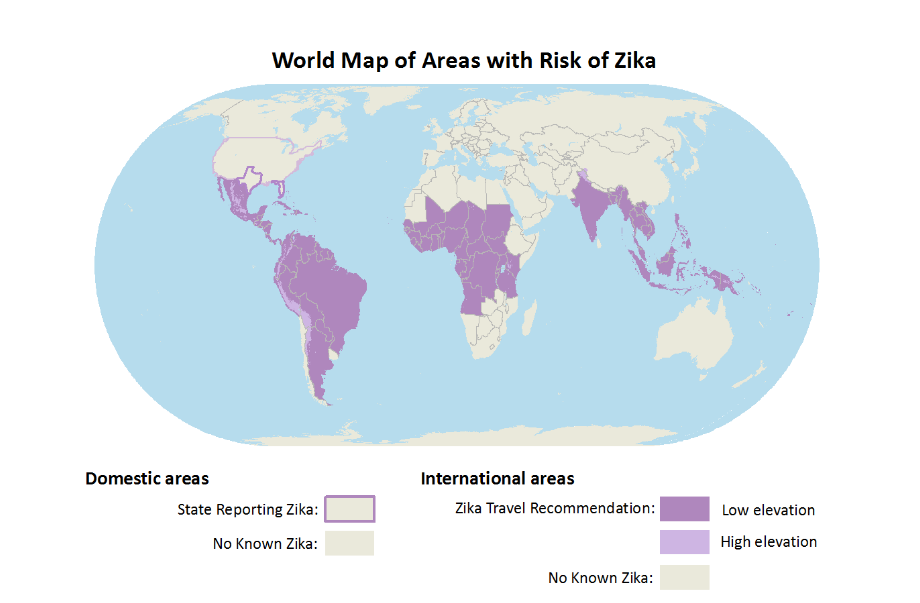
\includegraphics[scale=0.5]{images/map_zika.png} 
\caption{Countries with Zika Virus: Source CDC}\label{fig 1}
\end{figure}


Zika virus is mainly spread by Aedes mosquitoes. When a pathogen carrying mosquito bites an uninfected individual it infects them with the virus.
Other ways  by which the virus spreads include,
blood transfusion, unprotected sex with an infected person and from mother to child, infected mothers can pass on the virus to their unborn children \citep{musso2014}.

Some of the symptoms of Zika virus  are papular rash,fever, arthritis or arthralgia \cite{musso2015}. Papular rash is  characterized by a flat, red area on the skin that is covered with small confluent bumps and arthralgia is characterised by pain or aching in the joints without pain.

In addition, headache and red eyes are common symptoms of Zika virus. \cite{simoes2016zika}  adds that the extent of the risk that Zika infection will result in birth defects still remains unknown. For expecting mothers, Zika virus affects their foetus and development of the baby. Babies can face a range of neurologic sequelae such as intellectual disability, hearing loss, vision loss, and seizures. These problems can range from mild to severe and are often life-long \citep{rasmussen2016zika}.

There is no known vaccination to prevent or treat the Zika virus. Prevention measures can be taken to prevent the spread of the virus. This can done by preventing mosquito bites. Measures such as sleeping under a mosquito net, using mosquito repellent and fumigating mosquito breeding areas in the vicinity among others can be taken. Another measure of prevention of Zika virus is practising safe sex and avoiding travel to areas with high prevalence of Zika.

Drugs for the symptoms of Zika are administered to patients as a way of treating Zika patients because of the lack of a vaccine for the virus.


The spread of Zika virus has resulted in Zika epidemics in some part of the world as can be seen in figure \ref{fig 1} above as of April 2017. This causes a worry as the effects of the epidemic are more devastating and if not controlled can affect the whole country, region and World at large. 


 \section{Epidemiology}
 
Epidemiology is the study of the origin and course of diseases in a community. The goal of epidemiologist is to understand the cause of a disease, then to predict its course, and come up with methods to control the disease. This involves collaborative work of statisticians, mathematicians, physicians and various health specialists \citep{Brauer2017}.

The knowledge about infectious diseases has been built up by the method of experience, by observation and analysis of particular conditions associated with occurrence of the disease in nature \citep{frost1923importance}.
 
The first step in epidemiology was the collection and analysis of data on causes of death in London parishes in the early 1660s by Graunt.
He  gave a method of estimating the comparative risks of dying from various diseases, giving the first approach to a theory of competing risks \citep{Brauer2017}.
 
Mathematical models of disease transmission have been used to link biological processes of disease transmission and emergence of dynamics of infections at  population level. Researchers try to understand the environmental, biological and behavioural infectiousness of a disease.

 Environmental infectiousness depends on geographical conditions of the area in which, an  infected person resides. Some pathogens cannot survive inside or outside a host in given geographical  conditions. Thus, some diseases or infections spread faster in certain weather conditions \citep{grass}.
Understanding the timing and causes of seasonality offers important insights on how parasite–host systems interact. How and when parasite control measures can be applied, and how disease risks will respond to anthropogenic climate change and altered patterns of seasonality \citep{altizer}. These factors must be captured in the models.

Biological infectiousness depends on the pathogen's life cycle and the individual's or host's immune system. Some individuals have a strong immunity against certain infections, this may slow down the propagation the infection. On the other hand the life cycle of pathogens also affects the transmission dynamics of the infection. Some pathogens can only survive in the host while the other can survive outside the host, this will play a major role in the spread of the infection. The interaction of the genetic determinant of disease propagation in the pathogen and host is important in building models for the transmission dynamics of infectious diseases.

Behavioural infectiousness depends on the interaction behaviour of an individual. The contact pattern of the person affects how the individual is likely to propagate the disease. Depending on the nature of disease transmission, a person who has a lot of contacts is are more likely to spread the disease to more people compared to one who has fewer contacts \citep{johnson2001sexual}. Contact in this context implies any interaction likely to result in transmission of an infection.

The susceptibility of an individual largely depends on the biological, environmental and behavioural factors of an individual. For example, one's contact pattern, immunity and the environmental conditions will highly affect the probability of contracting an infection.

For over a  century, mathematical representation and analysis of infectious diseases has been  the centre of  infectious disease epidemiology \citep{b2005}.

Mathematical modelling of infections diseases, started by the works of Daniel Bernoulli in \cite{bernoulli1760essai}, in the quest to model the spread of small box and possible eradication. A century later the modelling become well established. The modelling of infectious disease dynamics is important for science and public policy among others. There are three main aims of infectious disease modelling; to understand the how the spreading mechanism of the disease, to  predict how the disease will progress among the population and to understand how the disease can be controlled. They provide tools for investigating and quantifying the spread of disease. Conducting experimental research on the spread of infectious disease raises a lot of ethical issues and therefore can not be conducted on humans. Mathematical simulations and modelling the disease has helped in providing understanding of the impact of the infectious disease on the population and give a guide for new control measures \citep{ming2016stochastic}.


\section{Modelling Infectious Disease with Compartmental Models}

Differential equations have been used in the modelling of the dynamics of the spread of infectious diseases. They are based on the assumption of uniform mixing, that is, everyone in the population has an equal probability of contracting an infectious disease \citep{kaplan2002emergency}.
Compartmental Mathematical models have been used to describe the transmission dynamic of Zika Virus \citep{gao2016}. Infectious diseases are transmitted indirectly  or directly by contact between the infected and those who are not infected thus these models try to capture these interactions \citep{sat}. 
 
In compartmental models of infectious disease individuals are divided into  several compartments such as; Susceptible (S) , latent (E) , infected (I), vaccinated (V) and recovered or removed (R). Depending on the on the propagation of the disease, compartmental models are built by combining these different classes or creating new ones \citep{li}.

 
Deterministic models also known as compartmental describe and explains what happens on average of the population. They assume that the population is homogeneous, that is, everyone in the population reacts the same risks of exposure and infection. This assumption does not capture biological, environmental and geographical  factors that effect susceptibility of individuals. Hence, the introduction of stochastic models. Stochastic models introduce the idea of randomness in the reaction to risk and infection by individuals in the population \citep{ming2016stochastic}. The main advantage of the stochastic models is they take into consideration each individual, but the major drawback is that it is laborious to model them as they require a lot of stimulation and sometimes become mathematically complex.
 
Deterministic models are built on theories of ordinary differential equations, partial differential equations and difference equations \citep{keeling2008modeling}.
The trends in these research areas are for higher model dimension and deeper and more refined analysis. Unlike for stochastic models where the trends of research are
toward specific diseases and toward deterministic and stochastic mixed models \citep{fu2013propagation}.


 
 To build models that incorporate contact patterns of the individuals, Mathematicians have resolved  to use results from the work of \cite{moreno1945application}, where he analysed contact patterns of prisoners. This work has given basis for understanding or building models based on the contact patterns of individuals in the population \citep{sat}. \cite{freeman2004development} characterizes the analysis of social networks by four properties. First, it involves the intuition that links between social actors are important. Second, it is based on the collection and analysis of data about social relations that link actors. Third, it draws heavily on graphic imagery to reveal and display the patterning of those links and lastly, it develops mathematical and computational models to describe and explain those patterns. 
A number of disease propagation models have been built for various infectious diseases among others Malaria, Zika, HIV -AIDS, Smallpox  and Chickenpox \citep{ding2016mathematical}.


\section{Modelling Infectious Diseases on Graphs}
Graph theory has over the years grown and has found its application in many fields. A graph also known as a network can be defined as a pair $G = (V, E) $ where $V$ is a finite set of nodes $E \subset V \oplus V = \left\lbrace e_1,e_2,\dots, e_m \right\rbrace$ is a set \citep{estrada2012structure}.

Over the years contemporary science, has had challenges in describing complex networks. This posed limits in the advancement of many disciplines. However, with the advancement of computerization, there is a raise in the possibility of understanding the stability of large networks \cite{barabasi1999emergence}.

For many complex networks vertices are described as elements of the system and edges represent the interaction between them. Similarly, in modelling the spread of  infectious diseases on networks, individuals or populations are represented by nodes of the network, contacts likely to result in the transmission of disease are represented by edges. Modelling of infectious disease on networks give better models for heterogeneous populations \citep{ming2016stochastic}. One of the major challenges in modelling the spread of infectious diseases on networks, is capturing  the contact patterns of individuals. The non availability of such data has lead to mathematicians modelling the spread of infectious diseases on various simulated network structures \citep{pastor2001}.


 Random network models of infectious disease do not take into account spatial position of individuals and connections are made at random \citep{keeling2005networks}. The growth rate and and final epidemic size of a disease on a random network are reduced compared with a random mix model. Growth rate in random network is $\tau (n -2) - g$ and the growth rate with random mixing is $\beta - g = \tau \widehat{n} -g$ , where  $\tau$ is the transmission rate across a contact, $n$ and $\widehat{n}$, is the number of contacts in a network and the unit number of contact per unit time in a random mixing model respectively. $g$ is the probability of recovery.
 
The reduction in the growth rate is due to two reasons; each infectious individual has been infected by one of its contacts, reducing the number of susceptible $n-1$ and as an infectious individual starts to infect its susceptible contacts it depletes its local environment, regardless of the population prevalence rate, hence limits the rate of disease spread \citep{keeling2005networks}.

Lattice based epidemic models are used to study the spatial and temporal rates of the disease spread in  a spatially distributed host populations \citep{rhodes1997epidemic}. Models built on latices assume that individuals are located as nodes on a regular lattice and connections are made to a collection of near neighbours or each node. For example people may be spread out such that connections are made to their four nearest neighbours, one on the left,right, up and down. \citep{lloyd2006infection}. To avoid the effect of the nodes at the end not being connected the last and first neighbours are made neighbours. The spread of influenza is one of the infectious disease that have been modelled based on lattice models \citep{liccardo2013lattice}. 

Another kind of network epidemic model has been the small world network. Disease spread through small-world networks has received considerable attention from both a theoretical and more applied context. The high level of clustering means that most infection occurs locally,  but short path lengths mean that epidemic spread through the net-work is rapid and disease is unlikely to be contained within small regions of the population \citep{watts1998collective}.

The spread of infectious diseases on network has also has also been modelled on scale free networks. Infectious disease like Ebola, SARS and HIV-AIDS have been modelled on scale free networks. A scale free network is a network whose degree distribution follows a the power that is $P(k) \approx ck^{-\lambda}$  \citep{morita2016six}


Simulated network models have been used to model the spread of disease, whose network data is difficult to collect. Various infectious diseases have been modelled on simulated networks \citep{keeling2005networks}. Networks that are based on simulation are limited because they are no ways to test the sensitivity of the epidemiological results to the details of the network structure. Nevertheless, a range of idealized networks and analytical tools that can reveal elements of network structure that are important determinants of epidemic dynamics, have been developed \citep{keeling2005networks}. 

A number of infectious disease models have been built on various network structures. This is so because networks capture the contact patterns in a community. The networks are either social networks or simulated networks. Many real world and social networks in which infectious diseases propagate is either small world or scale free networks and not random or regular as earlier assumed \cite{watts1998collective}. The underlying structure of a network influences  the effect of that the dynamics of epidemics will have on a population. For example in a small world network, where the network has a high clustering coefficient a shorter average distance. A disease is more likely to spread faster than in a random network or a regular network \citep{watts1998collective}.



